\documentclass[12pt, a4paper]{article}

% =============================================================
% PACKAGES
% =============================================================

% --- Encoding & Language ---
\usepackage[utf8]{inputenc}
\usepackage[T1]{fontenc}
\usepackage[english]{babel}

% --- Page Layout ---
\usepackage[a4paper, margin=2.5cm]{geometry}

% --- Typography ---
\usepackage{microtype}          % Microtypography: protrusion & font expansion
\usepackage[parfill]{parskip}   % Paragraph spacing instead of indentation

% --- Math ---
\usepackage{amsmath}
\usepackage{amssymb}

% --- Graphics & Floats ---
\usepackage{graphicx}
\usepackage{float}

% --- Tables ---
\usepackage{booktabs}

% --- Lists ---
\usepackage{enumitem}

% --- Colors (required before hyperref for named colors) ---
\usepackage[dvipsnames]{xcolor}

% --- Hyperlinks & PDF Metadata ---
\usepackage{hyperref}
\hypersetup{
    colorlinks = true,
    linkcolor  = MidnightBlue,
    citecolor  = MidnightBlue,
    urlcolor   = MidnightBlue,
    pdftitle   = {Practical Assignment Report: Time Series Segmentation},
    pdfauthor  = {Jesus Fernandez Lopez and Rafael Carlos Schoettel Vilchez},
    pdfsubject = {Metaheuristics},
    pdfkeywords= {time series segmentation metaheuristics hill climbing simulated annealing},
}

% =============================================================
% GLOBAL DOCUMENT SETTINGS
% =============================================================

% Prevent orphan and widow lines
\widowpenalty  = 10000
\clubpenalty   = 10000

% Consistent sentence spacing (one space after periods)
\frenchspacing

% --- Metadata Macros ---
\newcommand{\reporttitle}{Time Series Segmentation}
\newcommand{\reportdate}{March 15, 2026}
\newcommand{\authorA}{Jes\'{u}s Fern\'{a}ndez L\'{o}pez}
\newcommand{\authorB}{Rafael Carlos Schoettel Vilchez}

% =============================================================
\begin{document}
% =============================================================

% --- Title Page ---
\begin{titlepage}
  \centering
  \vspace*{3cm}

  {\Huge \textbf{Practical Assignment Report}}\\[0.8cm]
  {\LARGE \textbf{\reporttitle}}\\[0.5cm]
  \rule{\textwidth}{0.4pt}\\[2cm]

  {\Large \textbf{Authors}}\\[0.4cm]
  {\large \authorA\ \& \authorB}\\[1.5cm]

  {\Large \textbf{Course}}\\[0.4cm]
  {\large Metaheuristics}\\[0.4cm]
  {\normalsize Universidad de Córdoba}\\[1.5cm]

  {\Large \textbf{Date}}\\[0.4cm]
  {\large \reportdate}

  \vfill
  \rule{\textwidth}{0.4pt}
\end{titlepage}

\newpage
\tableofcontents
\newpage

% =============================================================
\section{Problem Formulation}
% =============================================================

The goal is to segment a time series into $k$ segments. For each segment, a linear
regression must be fitted using all the points within that segment. The aim is to
determine the $k$ segments (i.e., the bounds of each segment) that minimise the
average Mean Squared Error across all segments.

\begin{itemize}[itemsep=0.3em]
  \item \textbf{Solution Representation:} A solution is defined as an array of $k-1$
        sorted integers representing the indices (time steps) at which the series is split.

  \item \textbf{Objective Function (Fitness):} Minimise the Average Mean Squared Error
        across the $k$ segments. For each segment, a linear regression ($y = mx + b$) is
        fitted and its residual error is evaluated:
        \begin{equation}
          \mathrm{MSE} = \frac{1}{n} \sum_{i=1}^{n} \bigl(y_i - \hat{y}_i\bigr)^{2}.
        \end{equation}
        The total cost of a solution is the arithmetic mean of the individual segment MSEs.

  \item \textbf{Constraints:}
        \begin{enumerate}[itemsep=0.2em]
          \item Split points must lie strictly within the series bounds ($0 < \text{split} < N$).
          \item No duplicate split points are allowed within the same solution.
          \item Split points must be sorted in ascending order.
        \end{enumerate}
\end{itemize}

% =============================================================
\section{Algorithms: Definition and Parameter Fine-Tuning}
% =============================================================

Before detailing how the search space is navigated, it is necessary to define the
three algorithms applied in this study and the methodology used to tune their
parameters for optimal performance across different time series (TSx).

\subsection{Random Search (RS)}
\textbf{Definition:} An uninformed algorithm that uniformly samples the search space.
Instead of exploiting a known neighbourhood, it generates a completely new, independent
random solution at each iteration.

\subsection{Hill Climbing (HC) --- Steepest Ascent}
\textbf{Definition:} A purely exploitative local search strategy. At each step, it
exhaustively evaluates all possible neighbouring solutions and strictly transitions to
the neighbour that provides the greatest reduction in MSE.

\subsection{Simulated Annealing (SA)}
\textbf{Definition:} A probabilistic metaheuristic inspired by the annealing process
in metallurgy. It avoids premature convergence by occasionally accepting transitions to
worse solutions. This acceptance is governed by the Metropolis Criterion
($P = e^{-\Delta E/T}$), which depends on a \emph{temperature} parameter that
decreases over time according to a cooling schedule.

% =============================================================
\section{Solution Generation and Neighbourhood Structure}
% =============================================================

To navigate the search space (composed of all valid combinations of $k-1$ split
points), it is essential to define how solutions are built and how the algorithm moves
between them.

\subsection{Random Initial Solution}
To begin the search, we generate an initial solution $S_0$. We randomly select $k-1$
unique points within the available range $[1, N-1]$ and sort them in ascending order.
This ensures that all points have the same initial probability of being chosen, avoiding
any bias in the initial segment sizes.

\subsection{Concepts of Neighbour, Neighbourhood, and Movement Operator}
In combinatorial optimisation, a \textbf{neighbour} ($S'$) is a new solution obtained
by applying a small modification to the current solution ($S$). The
\textbf{neighbourhood} is the complete set of all valid neighbours reachable in a
single step from the current state.

To generate these neighbours, we have designed an \textbf{Atomic Movement Operator
  ($\Delta$\nobreakdash-move)}. The operation consists of choosing a single split point
$s_i$ from the current solution and shifting it by an integer distance $\Delta$.

\begin{itemize}[itemsep=0.3em]
  \item The magnitude of $\Delta$ is bounded by a maximum-variability parameter
        (\texttt{max\_var}), empirically set to 1\% of the total number of points $N$.
        Thus $\Delta \in [-\texttt{max\_var},\, +\texttt{max\_var}]$, with $\Delta \neq 0$.

  \item \textbf{Validity Constraints:} For the neighbour to be valid, the new split
        point ($s_i + \Delta$) must satisfy $0 < s_i + \Delta < N$ and must not coincide
        with any existing split point in the solution.
\end{itemize}

\subsection{Practical Example of the Operator}
Consider a time series of $N = 300$ points divided into $k = 3$ segments (requiring
$k-1 = 2$ split points). Suppose the current solution is $S = [50,\, 150]$. With
$\texttt{max\_var} = \lfloor 0.01 \times 300 \rfloor = 3$, the operator evaluates
\textbf{every integer $\Delta \in [-3, 3] \setminus \{0\}$}, systematically generating
the following complete \textbf{neighbourhood}:

\begin{enumerate}[itemsep=0.2em]
  \item \textbf{Movements applied to the first split point (50),
          $\Delta \in \{-3, -2, -1, 1, 2, 3\}$:}
        \begin{itemize}[itemsep=0.15em]
          \item $\Delta = -3 \;\rightarrow\; S'_1  = [47,\; 150]$
          \item $\Delta = -2 \;\rightarrow\; S'_2  = [48,\; 150]$
          \item $\Delta = -1 \;\rightarrow\; S'_3  = [49,\; 150]$
          \item $\Delta = +1 \;\rightarrow\; S'_4  = [51,\; 150]$
          \item $\Delta = +2 \;\rightarrow\; S'_5  = [52,\; 150]$
          \item $\Delta = +3 \;\rightarrow\; S'_6  = [53,\; 150]$
        \end{itemize}
  \item \textbf{Movements applied to the second split point (150),
          $\Delta \in \{-3, -2, -1, 1, 2, 3\}$:}
        \begin{itemize}[itemsep=0.15em]
          \item $\Delta = -3 \;\rightarrow\; S'_7  = [50,\; 147]$
          \item $\Delta = -2 \;\rightarrow\; S'_8  = [50,\; 148]$
          \item $\Delta = -1 \;\rightarrow\; S'_9  = [50,\; 149]$
          \item $\Delta = +1 \;\rightarrow\; S'_{10} = [50,\; 151]$
          \item $\Delta = +2 \;\rightarrow\; S'_{11} = [50,\; 152]$
          \item $\Delta = +3 \;\rightarrow\; S'_{12} = [50,\; 153]$
        \end{itemize}
\end{enumerate}

In a single step, the neighbourhood is deterministically composed of these 12 distinct
solutions, demonstrating that the operator explores the entire integer range rather than
only its boundaries.

\subsection{Application of the Operator by Algorithm}
The way each algorithm interacts with this operator defines its exploration and
exploitation strategy:

\begin{itemize}[itemsep=0.3em]
  \item \textbf{Random Search (RS):} \emph{Does not use the movement operator or the
          concept of a neighbourhood.} At each iteration it discards the current solution and
        generates a completely new solution $S'$ from scratch. It performs blind global
        sampling without exploiting any local information.

  \item \textbf{Hill Climbing --- Steepest Ascent:} Uses the operator to generate and
        evaluate the \textbf{entire neighbourhood} at each iteration. In the previous
        example, it would evaluate all 12 generated neighbours and strictly select the one
        that minimises MSE. If no neighbour improves upon $S$, the algorithm concludes that
        a local optimum has been reached and terminates.

  \item \textbf{Simulated Annealing (SA):} Uses the operator to generate a
        \textbf{single random neighbour} per iteration. It randomly selects one split point
        and applies a random $\Delta$ from the allowed range (e.g., selects point 150 and
        applies $+2$, producing only $S'_{11}$). The decision to accept this new solution
        is governed by the Metropolis Criterion, allowing the algorithm to temporarily
        accept a worse MSE in order to escape local minima in a temperature-controlled
        manner.
\end{itemize}

% =============================================================
\section{Parameter Fine-Tuning and Experimental Setup}
% =============================================================

To ensure a fair and rigorous comparison between the metaheuristics, a preliminary
study was conducted to fine-tune each algorithm's parameters. The primary goal was to
find the optimal balance between solution quality (measured by MSE) and computational
cost for each specific time series.

\subsection{Random Search (RS): Convergence Analysis}

As a purely stochastic algorithm with no heuristic guidance, Random Search relies
entirely on the volume of iterations to find high-quality solutions. To avoid an
arbitrary stopping criterion, a multi-run convergence study was performed.

The algorithm was executed multiple times; the average best MSE at each iteration was
tracked to mitigate the impact of random variance. The theoretical optimal stopping
point was identified as the iteration where the average convergence curve exhibited
clear asymptotic behaviour (reaching within a 2\% tolerance of the absolute minimum
found).

The empirical optimal average stops were 6{,}869, 9{,}021, 4{,}369, and 3{,}445
iterations for TS1, TS2, TS3, and TS4, respectively.

However, relying strictly on the exact average limit leaves the algorithm vulnerable to
premature termination in exceptionally unlucky runs. Therefore, a deliberate safety
margin was added. The final stopping criteria adopted were:

\begin{itemize}[itemsep=0.2em]
  \item \textbf{TS1} ($k=9$):  7{,}000 iterations.
  \item \textbf{TS2} ($k=10$): 9{,}250 iterations.
  \item \textbf{TS3} ($k=20$): 4{,}500 iterations.
  \item \textbf{TS4} ($k=50$): 3{,}600 iterations.
\end{itemize}

\begin{figure}[H]
  \centering
  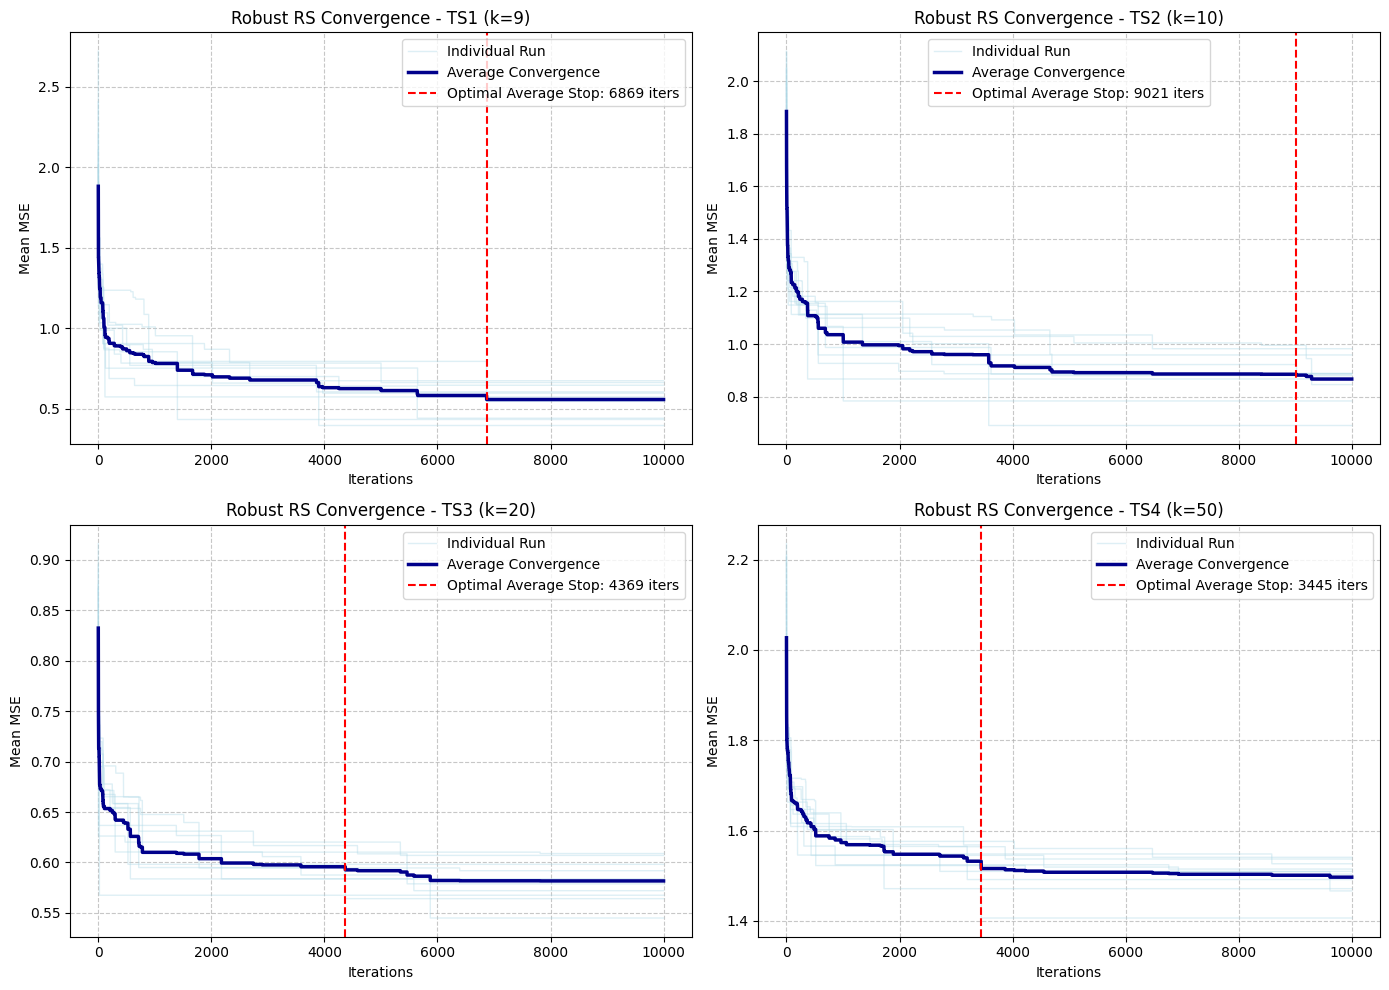
\includegraphics[width=0.85\textwidth]{img/RS-Stop.png}
  \caption{Random Search multi-run average convergence analysis.}
  \label{fig:rs_tuning}
\end{figure}

\subsection{Hill Climbing (HC): Independent Restarts Strategy}

Hill Climbing is a strictly exploitative local search algorithm. Once initialised, its
deterministic nature ensures it will rapidly descend into the nearest local optimum,
where it becomes permanently trapped. Consequently, internal parameter tuning (e.g.,
cooling rates) is not applicable to its core mechanism.

To evaluate its true capability as a global optimiser, a multi-restart strategy was
implemented. The central design question was determining how many random initialisations
are required to sufficiently sample different valleys of the search space.

A preliminary study tracked the cumulative best MSE across sequential independent
restarts. To avoid subjective visual estimation, a strict mathematical tolerance
threshold was applied: the optimal stopping point was defined as the exact number of
restarts for which the marginal improvement falls below 1\% of the absolute minimum
found across all trials.

This mathematically rigorous approach guarantees that the algorithm has extensively
explored the search space and converged to a near-global optimum. The final restart
configurations were:

\begin{itemize}[itemsep=0.2em]
  \item \textbf{TS1} ($k=9$):  18 restarts.
  \item \textbf{TS2} ($k=10$): 13 restarts.
  \item \textbf{TS3} ($k=20$): 9 restarts.
  \item \textbf{TS4} ($k=50$): 18 restarts.
\end{itemize}

\begin{figure}[H]
  \centering
  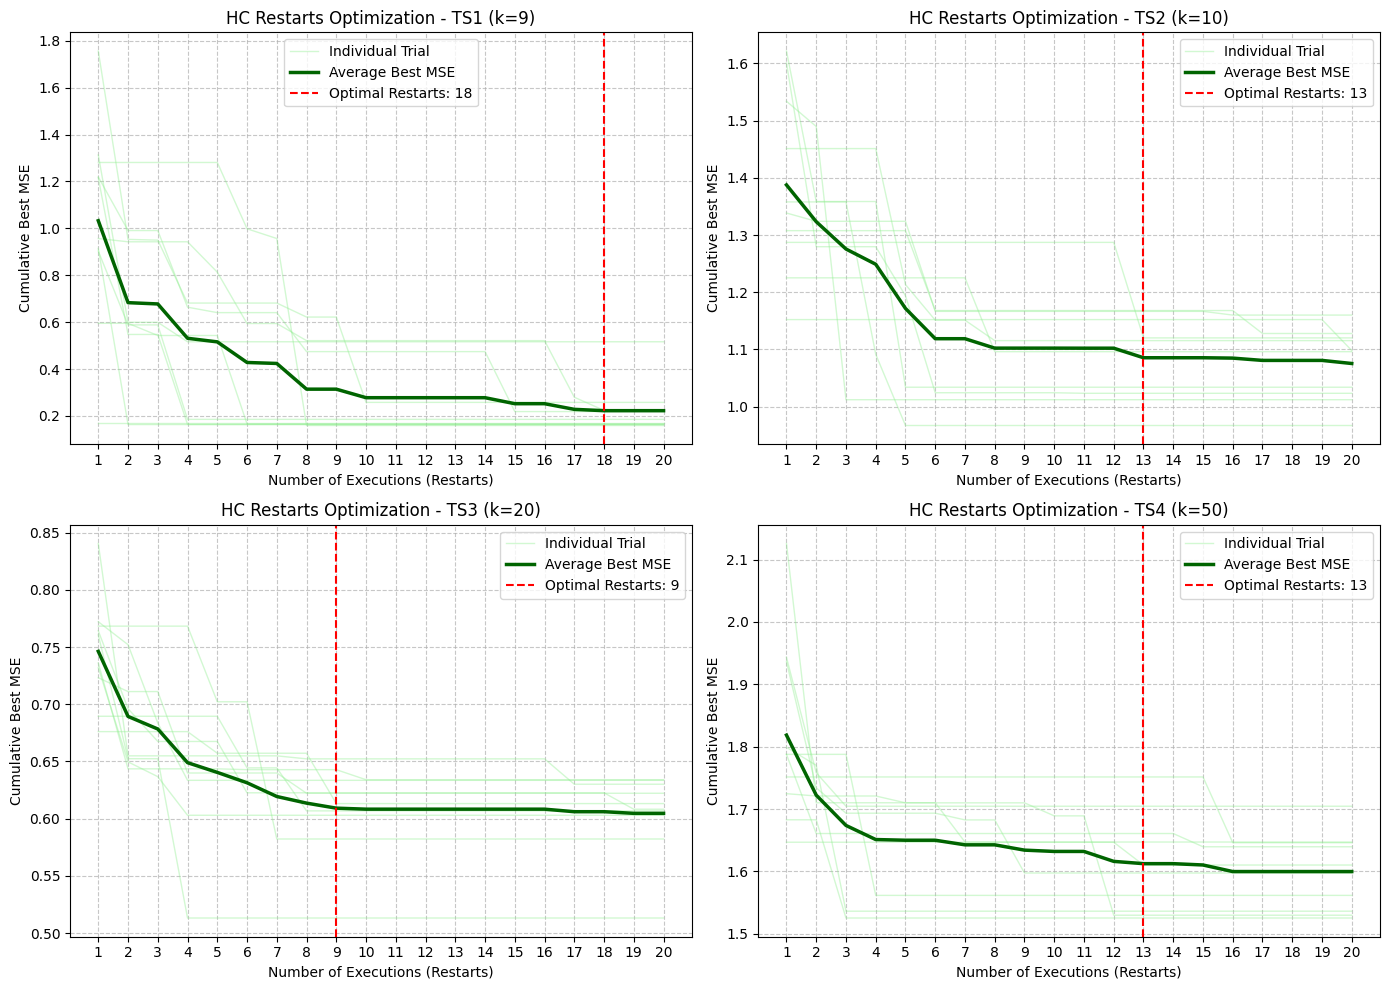
\includegraphics[width=0.85\textwidth]{img/HC-Restarts.png}
  \caption{Hill Climbing cumulative best MSE across independent restarts.}
  \label{fig:hc_tuning}
\end{figure}

\subsection{Simulated Annealing (SA): Grid Search Optimisation}

Simulated Annealing demands precise tuning of its cooling schedule to properly manage
the transition from broad exploration (high temperature) to strict exploitation (low
temperature). A robust Grid Search methodology was applied to determine the optimal
configuration.

The study evaluated Geometric and Linear cooling schedules across various initial
temperatures ($T_0 \in \{50, 100\}$), cooling rates ($\alpha \in \{0.95, 0.98, 0.99\}$
for geometric; step sizes $\{0.5, 1.0\}$ for linear), and epochs per temperature step
($L \in \{50, 100\}$).

\emph{Decision note: The Logarithmic cooling schedule, despite its theoretical
  guarantees of global convergence, was empirically excluded early in the process.
  Initial tests revealed that its extremely slow temperature reduction massively exceeded
  any reasonable computational time limits, rendering it impractical for these specific
  time series problems.}

Table~\ref{tab:grid_search} summarises the optimal parameter combinations discovered.
In all scenarios, the Geometric cooling schedule vastly outperformed the Linear
approach, providing a smoother transition to thermal equilibrium.

\renewcommand{\arraystretch}{1.3}
\begin{table}[H]
  \centering
  \caption{Optimal Simulated Annealing parameters obtained via Grid Search.}
  \label{tab:grid_search}
  \resizebox{\textwidth}{!}{%
    \begin{tabular}{lccccr}
      \toprule
      \textbf{Dataset}      & \textbf{Cooling}      & \textbf{$T_0$}    &
      \textbf{$\alpha$}     & \textbf{$L$ (Epochs)} & \textbf{Best MSE}                                \\
      \midrule
      \textbf{TS1} ($k=9$)  & Geometric             & 100               & 0.98 & 100 & \textbf{0.1591} \\
      \textbf{TS2} ($k=10$) & Geometric             & 50                & 0.98 & 100 & \textbf{0.8529} \\
      \textbf{TS3} ($k=20$) & Geometric             & 50                & 0.99 & 100 & \textbf{0.2293} \\
      \textbf{TS4} ($k=50$) & Geometric             & 100               & 0.99 & 100 & \textbf{0.4670} \\
      \bottomrule
    \end{tabular}}
\end{table}
\renewcommand{\arraystretch}{1}

The Grid Search results validate a core principle of metaheuristic design: parameter
selection is highly dependent on problem scale. While a high number of internal
evaluations ($L = 100$) proved beneficial across all datasets, the cooling rate
($\alpha$) varied with problem complexity. For larger search spaces (TS3 and TS4), the
algorithm systematically favoured a slower cooling rate ($\alpha = 0.99$) to prolong
thermal equilibrium. For simpler landscapes (TS1 and TS2), a faster rate
($\alpha = 0.98$) was sufficient without unnecessary computational overhead.

\begin{figure}[H]
  \centering
  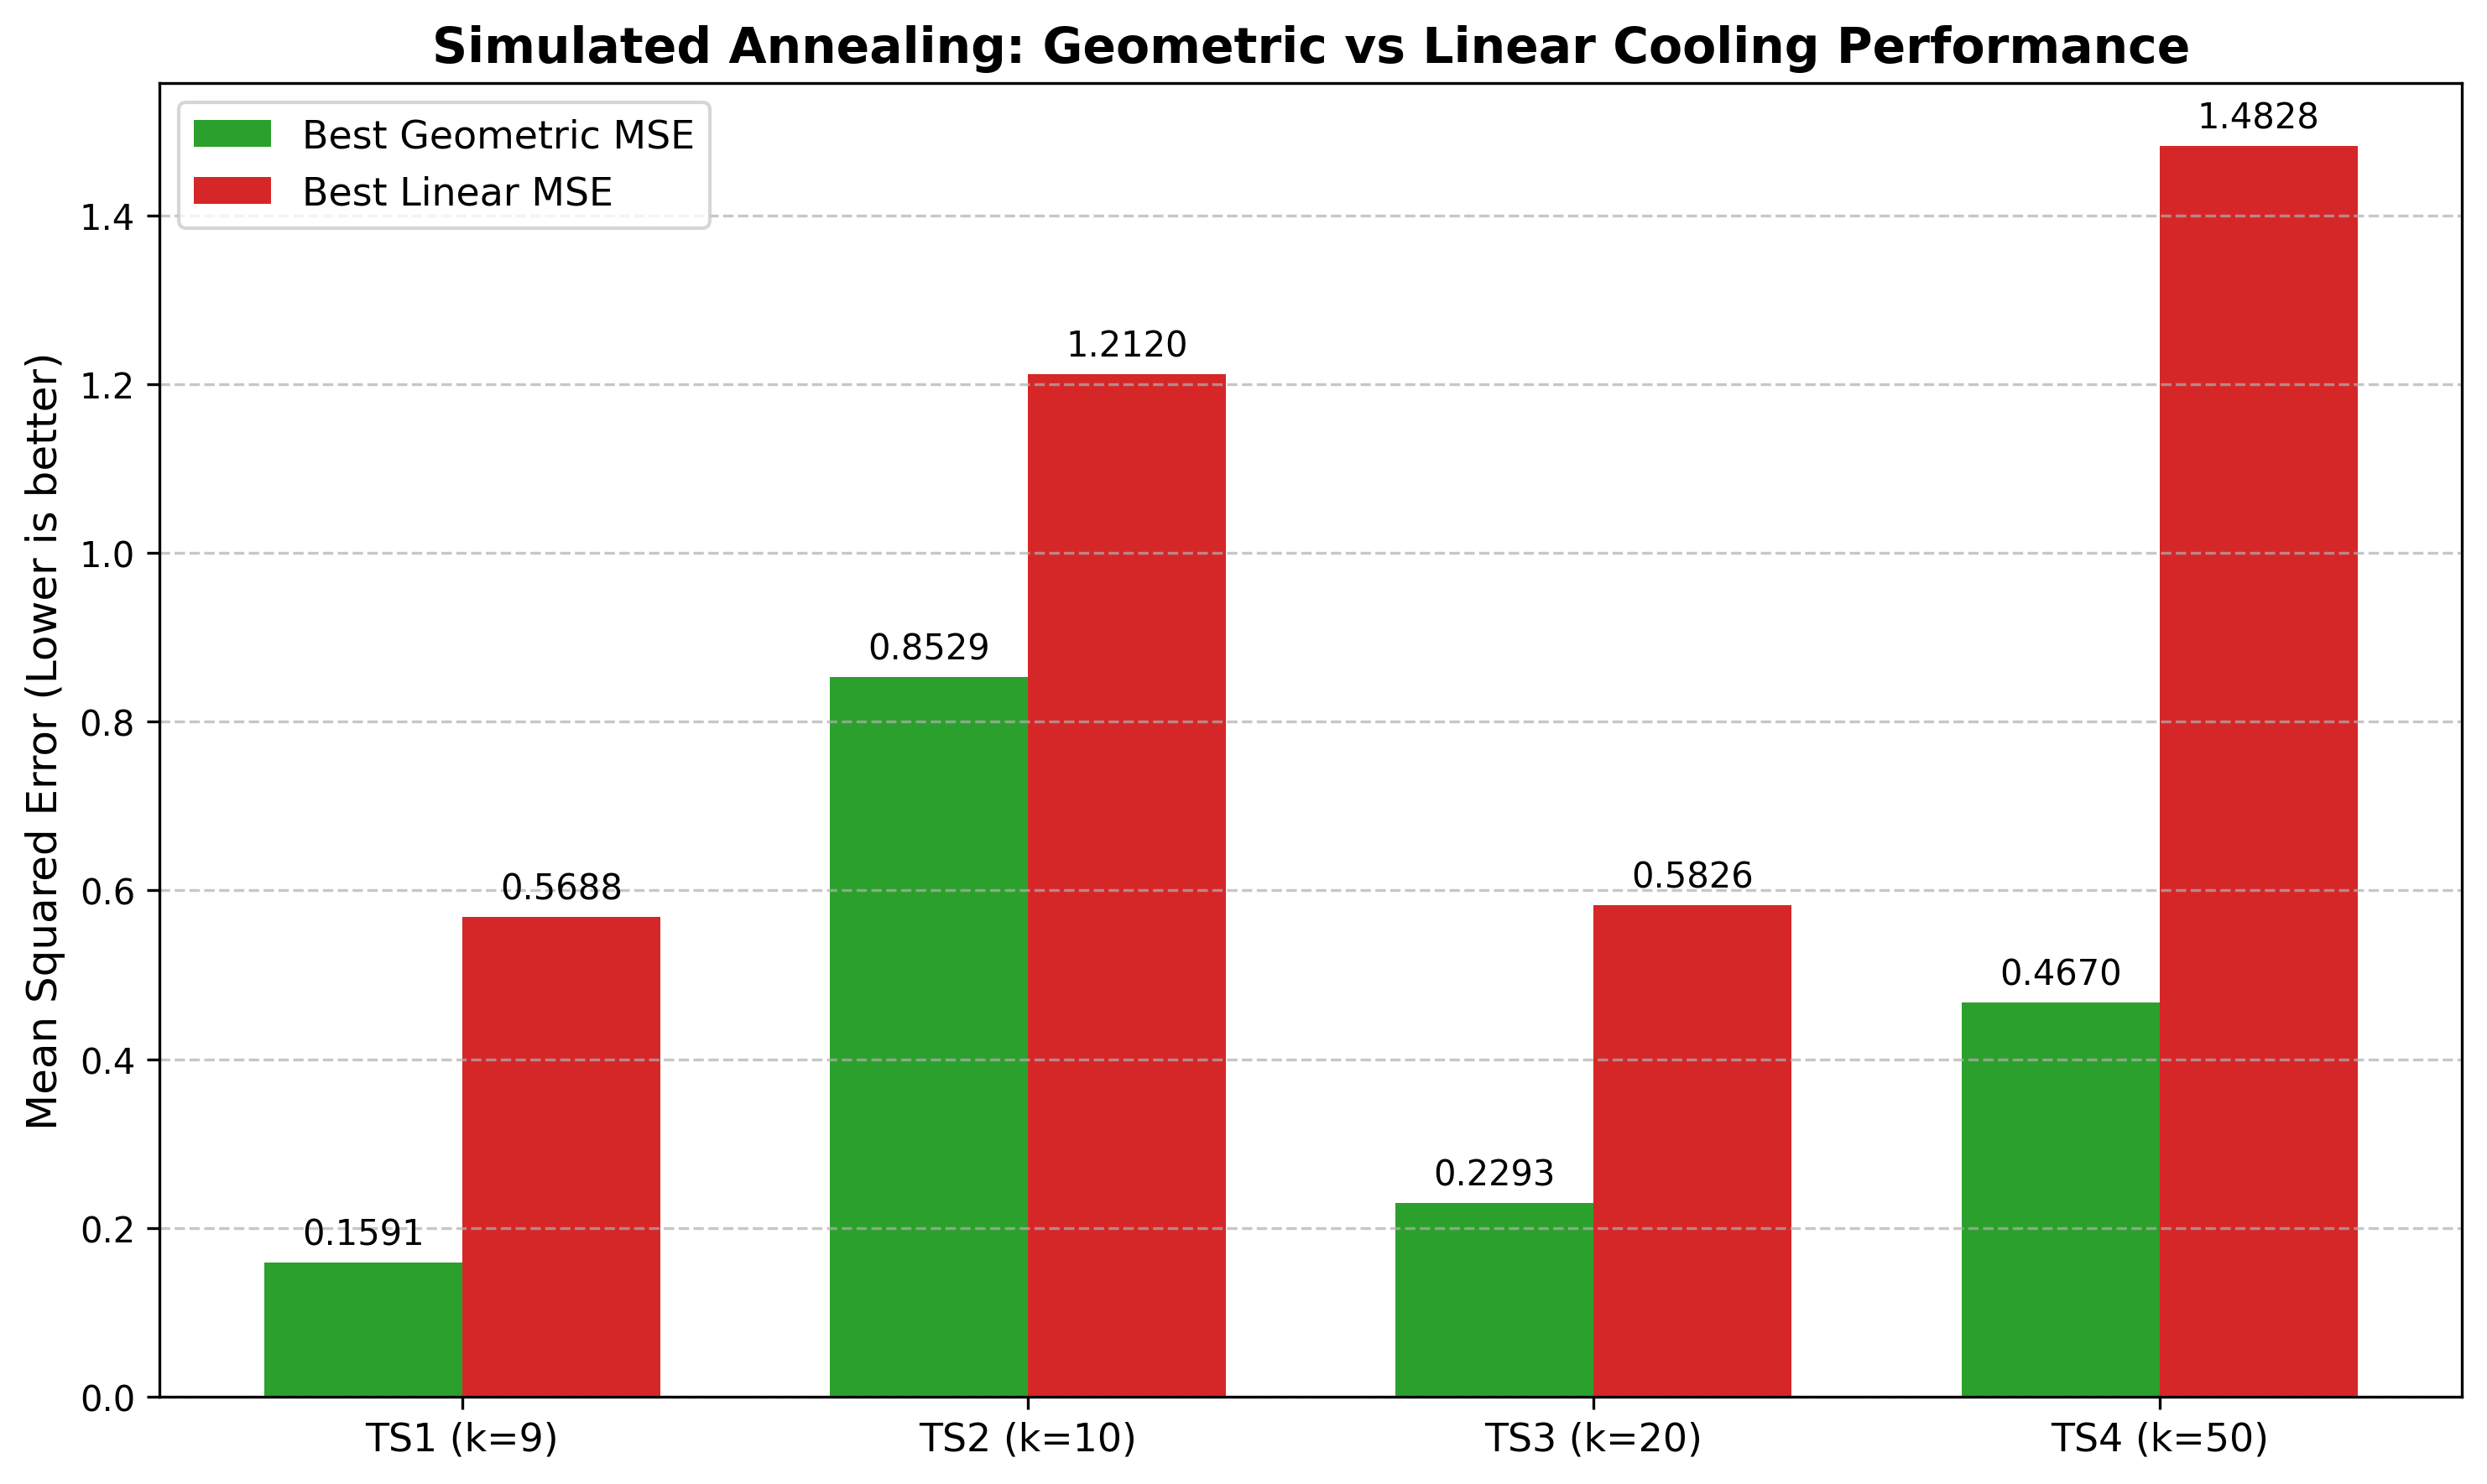
\includegraphics[width=0.85\textwidth]{img/SA-GEOvsLINEAR.png}
  \caption{Performance comparison: best Geometric vs.\ best Linear cooling MSE.}
  \label{fig:sa_cooling}
\end{figure}

% =============================================================
\section{Final Evaluation and Results}
% =============================================================

Following the rigorous fine-tuning phase, a final execution was performed using the
optimal parameters established for each algorithm. To determine the absolute best
segmentation for each time series, the algorithms were evaluated across multiple
independent runs, retaining only the single best solution found.

Table~\ref{tab:ultimate_summary} summarises the quantitative performance of the winning
algorithm for each dataset, illustrating the relationship between search space
dimensionality (defined by $k$) and algorithmic suitability.

\renewcommand{\arraystretch}{1.3}
\begin{table}[H]
  \centering
  \caption{Summary of the best solutions found across all datasets.}
  \label{tab:ultimate_summary}
  \resizebox{0.95\textwidth}{!}{%
    \begin{tabular}{lrcrr}
      \toprule
      \textbf{Dataset}  & \textbf{Segments ($k$)}     & \textbf{Winning Algorithm} &
      \textbf{Best MSE} & \textbf{Execution Time (s)}                                               \\
      \midrule
      \textbf{TS1}      & 9                           & Hill Climbing              & 0.1591 & 0.04  \\
      \textbf{TS2}      & 10                          & Simulated Annealing        & 0.8164 & 2.15  \\
      \textbf{TS3}      & 20                          & Simulated Annealing        & 0.2222 & 5.61  \\
      \textbf{TS4}      & 50                          & Simulated Annealing        & 0.4435 & 13.90 \\
      \bottomrule
    \end{tabular}}
\end{table}
\renewcommand{\arraystretch}{1}

As observed in the summary, Hill Climbing provides a remarkably fast and competitive
solution for lower-complexity landscapes (TS1). However, as the number of segments
increases (TS3 and TS4), Simulated Annealing consistently achieves the best results,
effectively navigating the combinatorial explosion at a naturally higher computational
cost.

The following figures visually present these best segmentations. Notably,
Figure~\ref{fig:ult_ts2} exposes the mathematical exploit discovered in TS2, where
Simulated Annealing clustered split points at the edges to artificially minimise the
unconstrained objective function.

\begin{figure}[H]
  \centering
  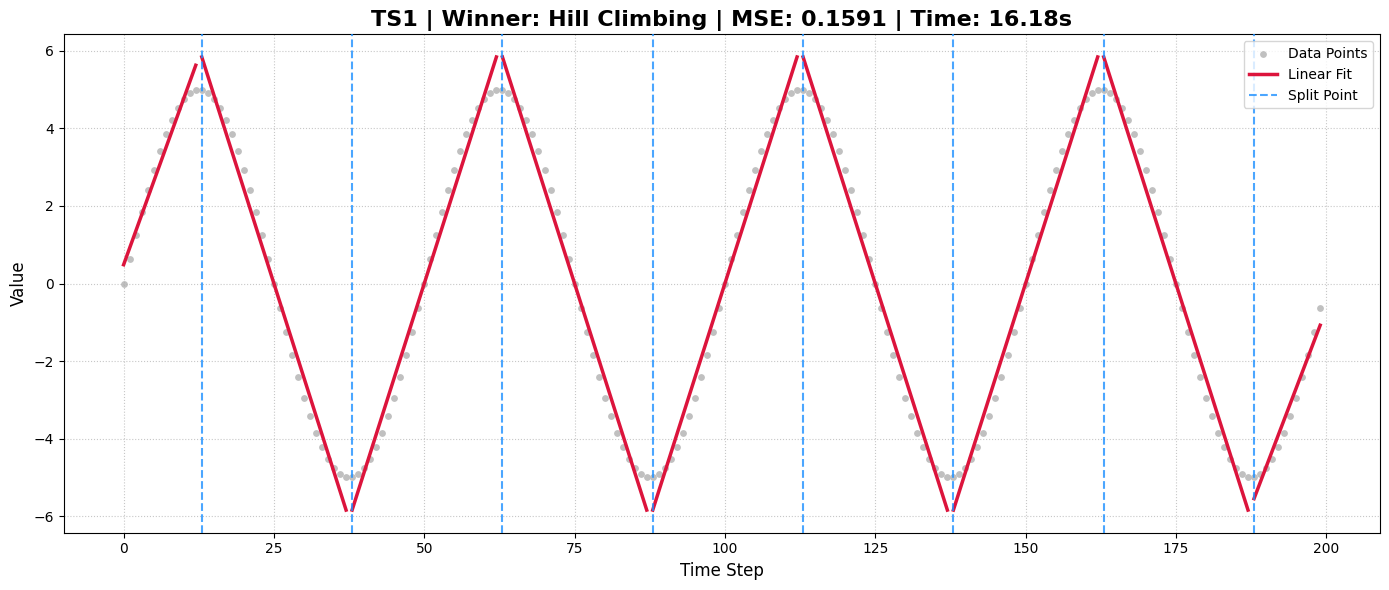
\includegraphics[width=0.9\textwidth]{img/Wts1.png}
  \caption{Best solution for TS1. Winner: Hill Climbing.}
  \label{fig:ult_ts1}
\end{figure}

\begin{figure}[H]
  \centering
  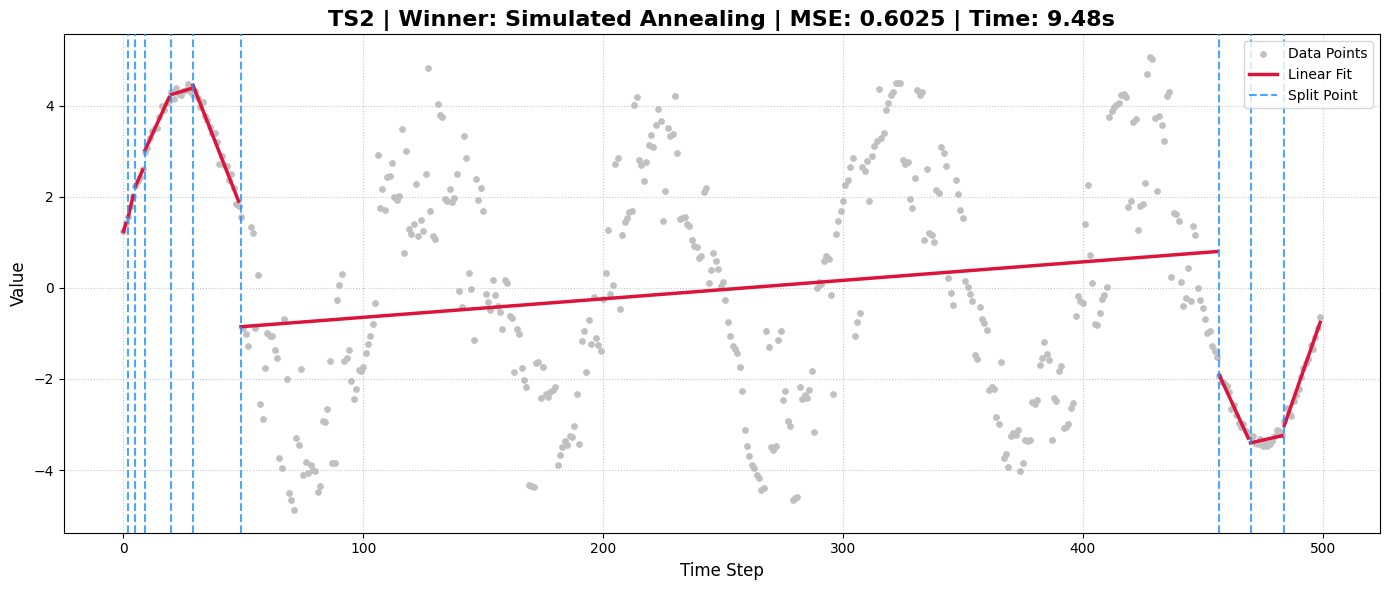
\includegraphics[width=0.9\textwidth]{img/Wts2.png}
  \caption{Best solution for TS2. Winner: Simulated Annealing
    (note the split-point clustering at the edges).}
  \label{fig:ult_ts2}
\end{figure}

\begin{figure}[H]
  \centering
  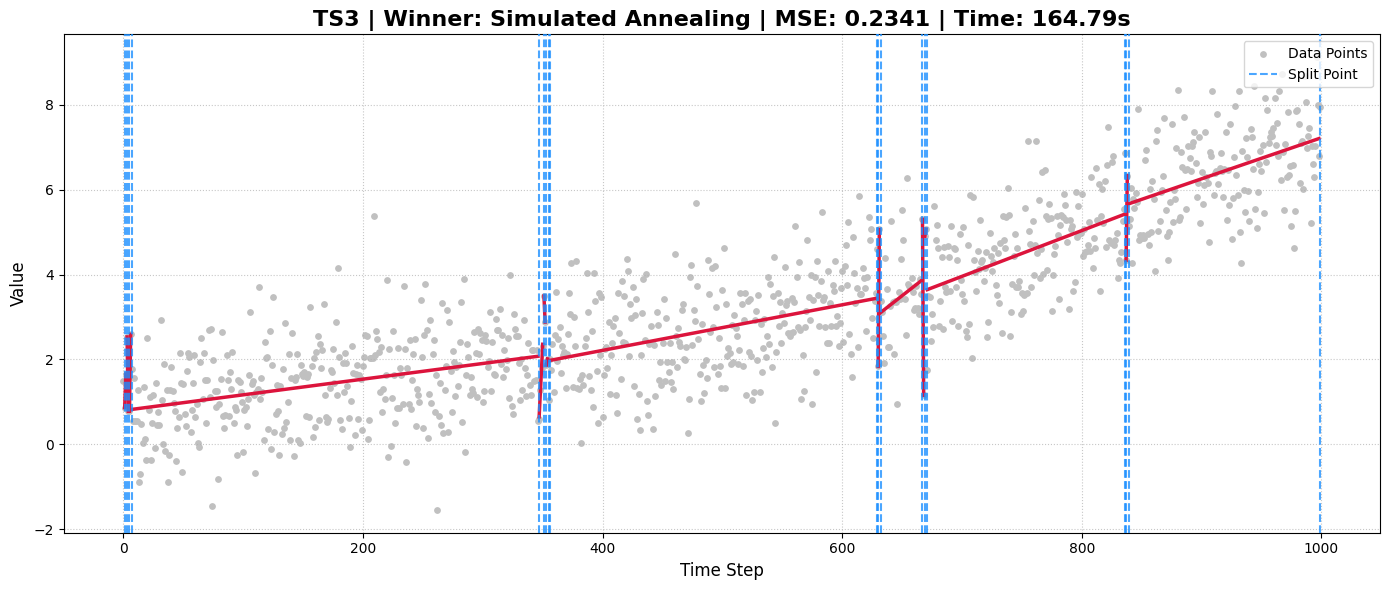
\includegraphics[width=0.9\textwidth]{img/Wts3.png}
  \caption{Best solution for TS3. Winner: Simulated Annealing.}
  \label{fig:ult_ts3}
\end{figure}

\begin{figure}[H]
  \centering
  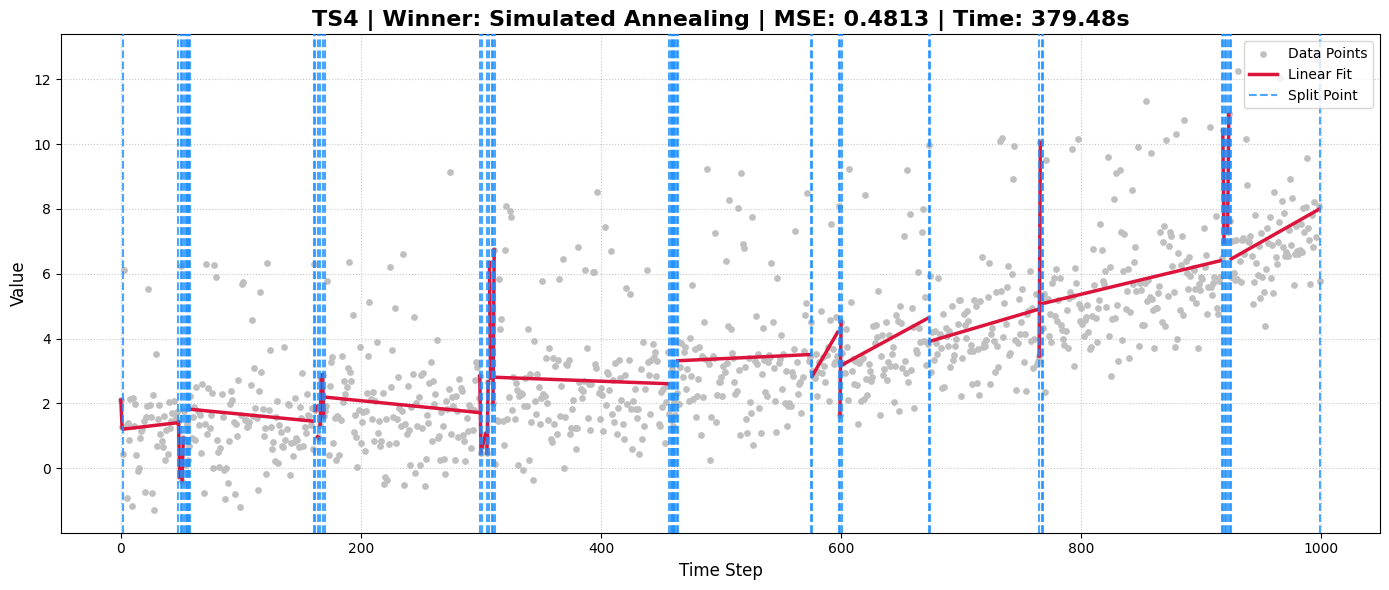
\includegraphics[width=0.9\textwidth]{img/Wts4.png}
  \caption{Best solution for TS4. Winner: Simulated Annealing.}
  \label{fig:ult_ts4}
\end{figure}

% =============================================================
\section{Conclusions and Critical Analysis}
% =============================================================

The experimental results yield two major conclusions regarding algorithmic scalability
and objective function design in time series segmentation.

\subsection{Algorithmic Scalability and Search Space Complexity}

In relatively simple optimisation problems with low dimensionality, such as TS1
($k = 9$), any well-implemented metaheuristic can perform adequately. In our final
trial, Hill Climbing achieved the lowest MSE (0.1591). However, in such constrained
spaces the performance difference is marginal: the ``winner'' could have equally been
Simulated Annealing or even Random Search, since success in low-complexity landscapes
is heavily influenced by stochastic initialisation rather than algorithmic superiority.

Conversely, as problem complexity scales exponentially (TS3 with $k = 20$ and TS4 with
$k = 50$), the behaviour changes drastically. Algorithms that lack a robust equilibrium
between \textit{intensification} (exploitation) and \textit{diversification}
(exploration) fail entirely. Hill Climbing repeatedly becomes trapped in sub-optimal
local minima due to its greedy nature; Random Search lacks the heuristic guidance to
refine boundaries. Simulated Annealing clearly dominates these high-dimensional
scenarios. Its thermodynamic cooling schedule and stochastic acceptance criterion
perfectly balance the exploration of new regions with the fine-tuning of local optima,
consistently securing the best MSEs.

\subsection{Objective Function Vulnerability: The ``MSE Hack''}

The results for TS2 (Figure~\ref{fig:ult_ts2}) expose a critical vulnerability in
relying solely on an unweighted arithmetic mean of MSEs as the fitness function. While
Simulated Annealing mathematically ``won'' by achieving an MSE of 0.8164, visual
inspection reveals that the resulting segmentation completely fails to represent the
actual curve of the data.

Because a linear regression fitted to one or two points yields an error of exactly
zero, the highly explorative SA algorithm effectively ``hacked'' the objective function.
It achieved this by clustering almost all split points at the extreme edges of the
dataset, creating numerous microscopic segments with zero error. Since the fitness
function calculates an unweighted arithmetic mean, these zero-error segments dragged
the overall average down, successfully masking the massive residual error of the single
oversized segment spanning the middle of the dataset.

\begin{figure}[H]
  \centering
  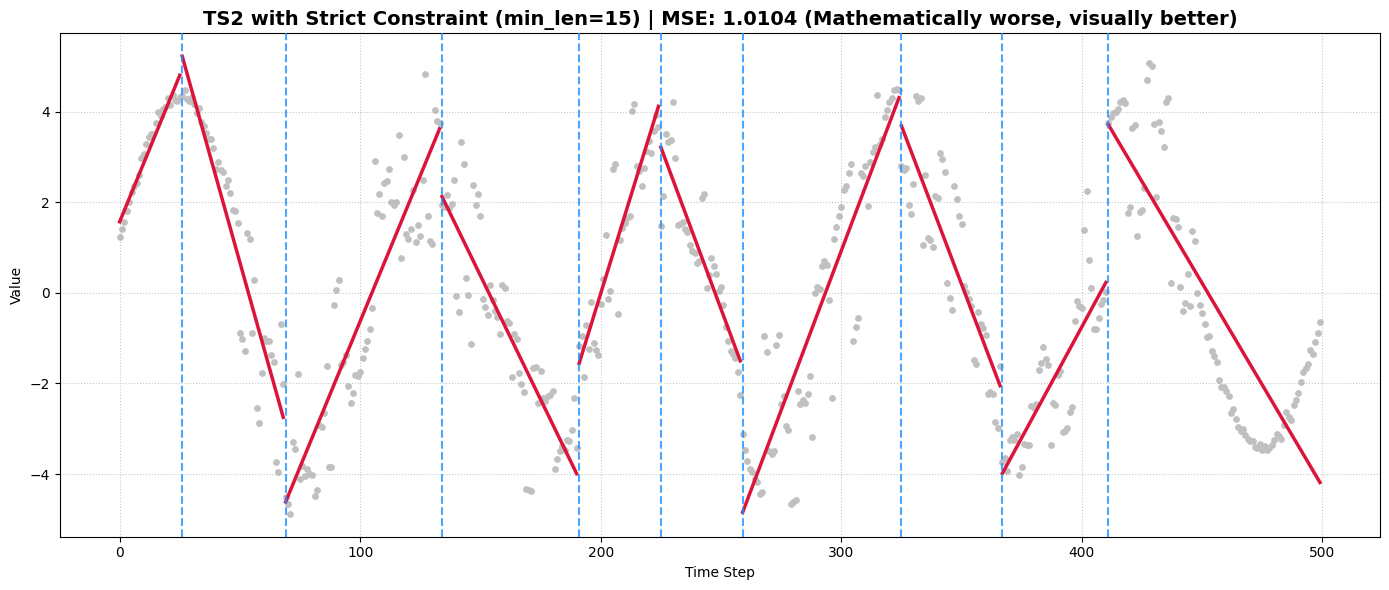
\includegraphics[width=0.9\textwidth]{img/MSEhackEXPLANATION.png}
  \caption{Visual proof of the objective function vulnerability. By enforcing a
    minimum segment length constraint (\texttt{min\_len}\,$= 15$), the
    algorithm is forced to follow the actual data curve. While this produces a
    visually superior and practically useful segmentation, it paradoxically
    yields a mathematically ``worse'' MSE (1.1098 vs.\ 0.8164).}
  \label{fig:mse_hack}
\end{figure}

To generate solutions that genuinely track the underlying data and prevent this exploit,
the fitness evaluation must be structurally constrained. Future implementations could
address this by:

\begin{enumerate}[itemsep=0.3em]
  \item Imposing a strict \textbf{minimum segment length} constraint during neighbour
        generation, forcing the algorithm to distribute cuts more evenly (as demonstrated in
        Figure~\ref{fig:mse_hack}).

  \item Replacing the arithmetic mean with a \textbf{geometric mean} or a
        \textbf{weighted average} based on the number of points in each segment, preventing
        tiny segments from disproportionately lowering the overall score.

  \item Incorporating \textbf{standard deviation penalties} into the fitness function,
        penalising solutions that exhibit extreme variance in segment sizes.
\end{enumerate}

% =============================================================
\section{Annex: Algorithmic Behaviour Visualisations}
% =============================================================

\emph{Note: The following visualisations were generated during early developmental
  phases, prior to optimal parameter tuning. While their quantitative metrics do not
  represent the final maximised performance of the algorithms, they are preserved here as
  qualitative examples of the inherent behavioural differences between purely stochastic
  exploration (Random Search), strict local exploitation (Hill Climbing), and balanced
  thermodynamic search (Simulated Annealing).}

\subsection{General Behaviour on TS1 ($k=9$)}
\begin{figure}[H]
  \centering
  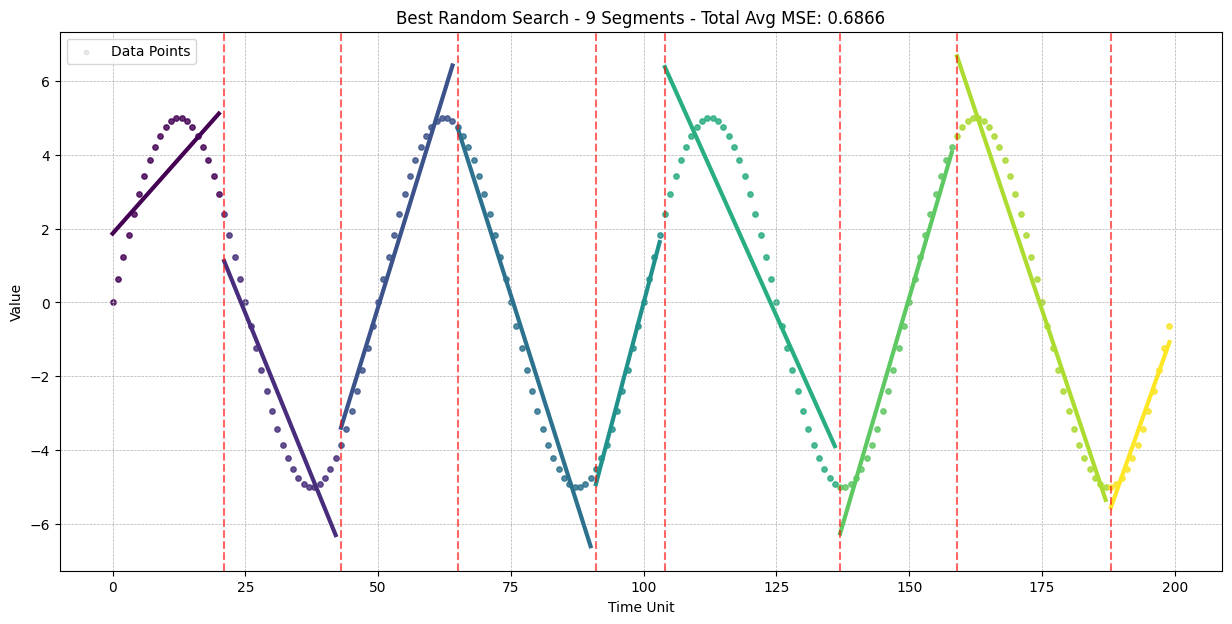
\includegraphics[width=0.85\textwidth]{img/RS-TS1.png} \\[0.3cm]
  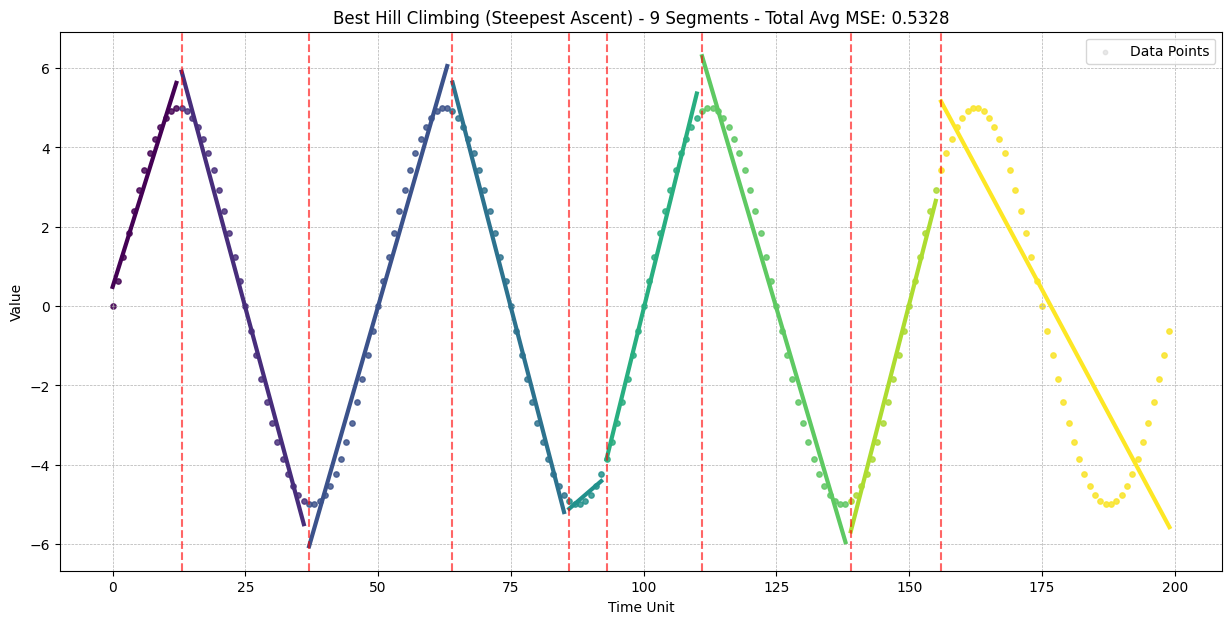
\includegraphics[width=0.85\textwidth]{img/HC-TS1.png} \\[0.3cm]
  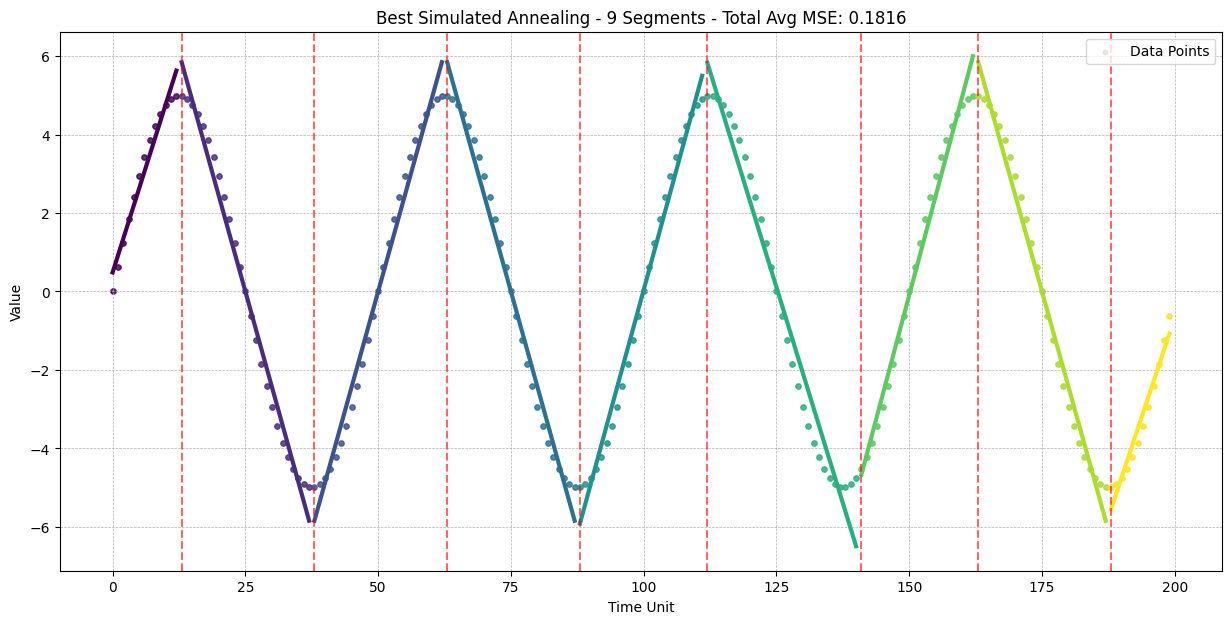
\includegraphics[width=0.85\textwidth]{img/SA-TS1.png}
  \caption{Behavioural comparison on TS1.
    Top: Random Search. Middle: Hill Climbing. Bottom: Simulated Annealing.}
  \label{fig:behav_ts1}
\end{figure}

\subsection{General Behaviour on TS2 ($k=10$)}
\begin{figure}[H]
  \centering
  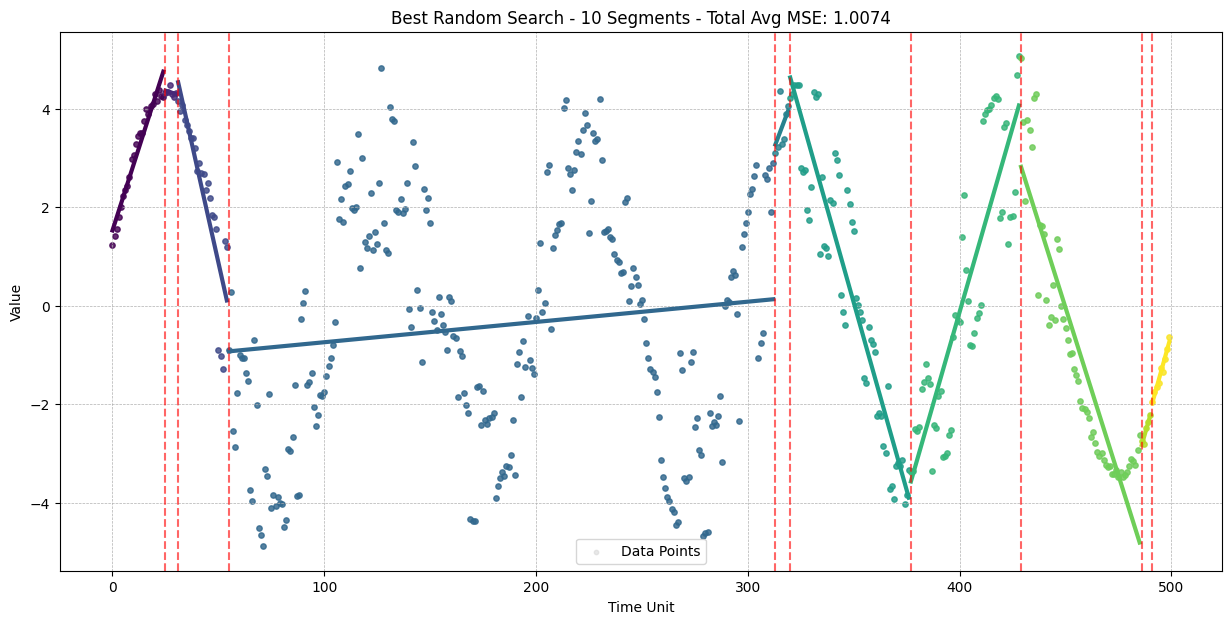
\includegraphics[width=0.85\textwidth]{img/RS-TS2.png} \\[0.3cm]
  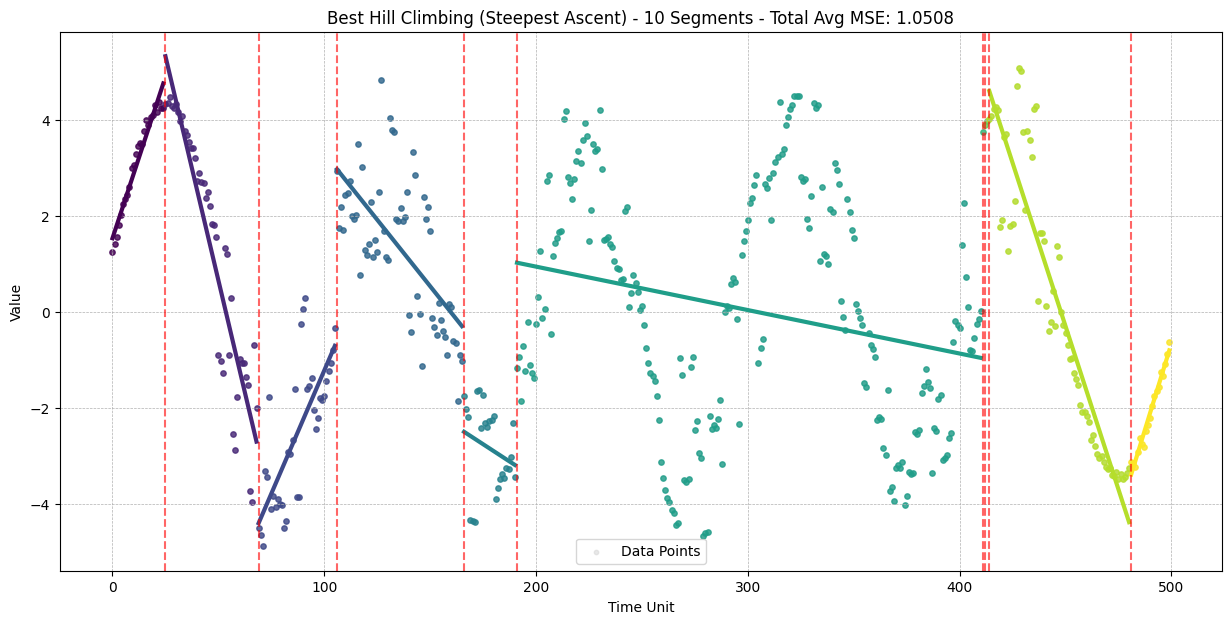
\includegraphics[width=0.85\textwidth]{img/HC-TS2.png} \\[0.3cm]
  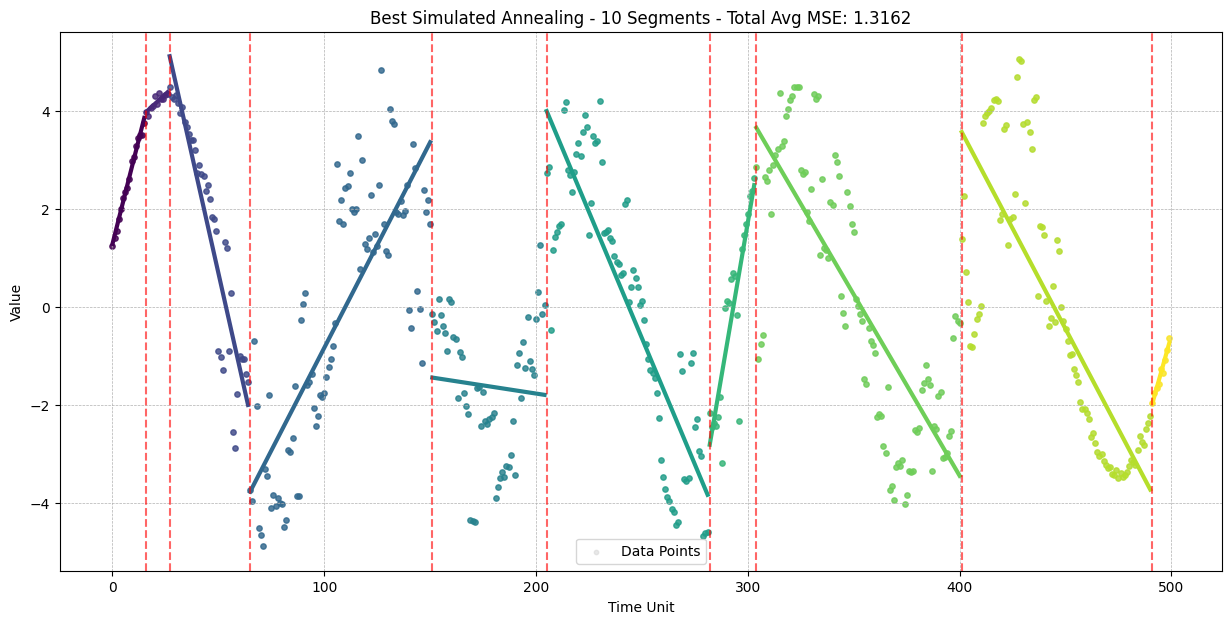
\includegraphics[width=0.85\textwidth]{img/SA-TS2.png}
  \caption{Behavioural comparison on TS2.
    Top: Random Search. Middle: Hill Climbing. Bottom: Simulated Annealing.}
  \label{fig:behav_ts2}
\end{figure}

\subsection{General Behaviour on TS3 ($k=20$)}
\begin{figure}[H]
  \centering
  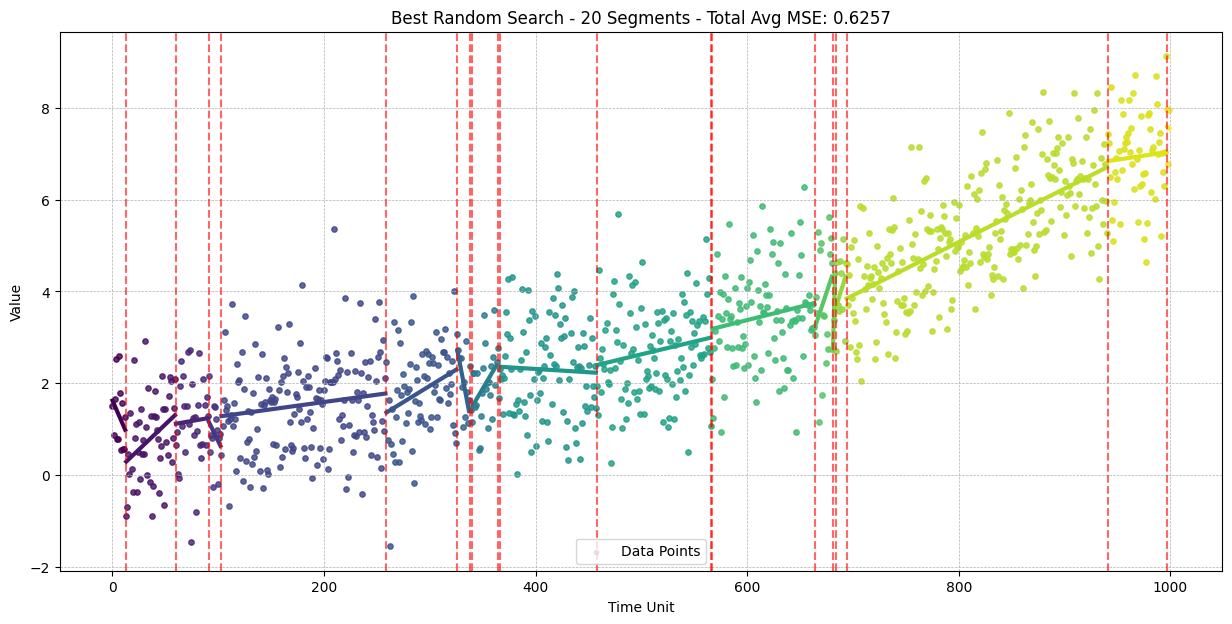
\includegraphics[width=0.85\textwidth]{img/RS-TS3.png} \\[0.3cm]
  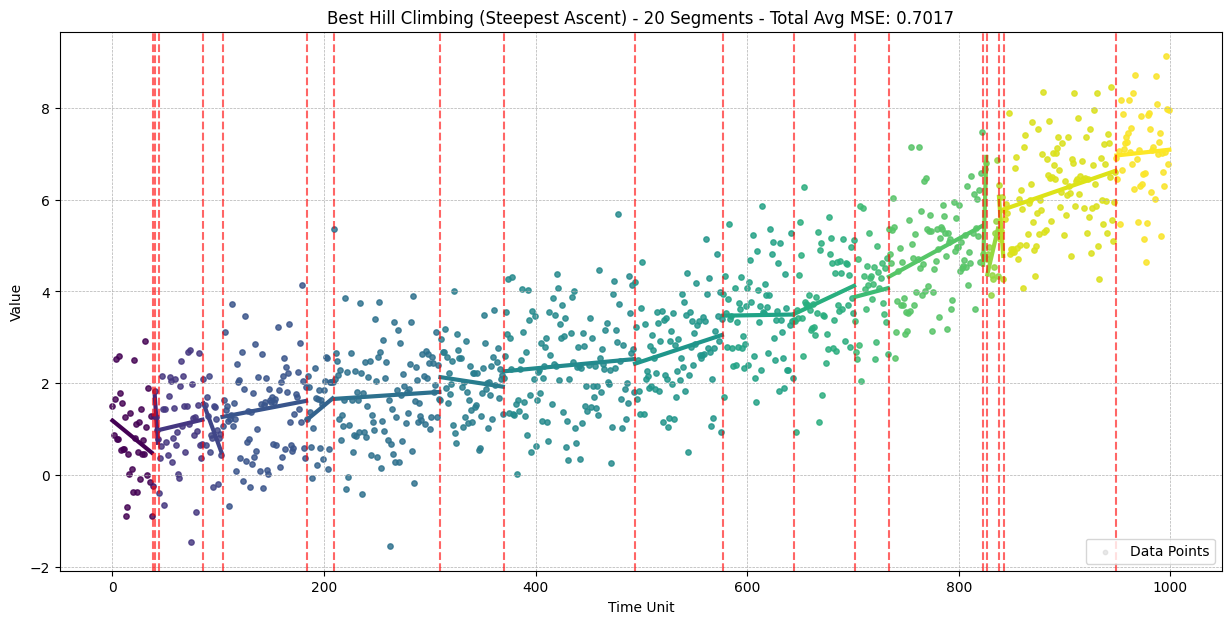
\includegraphics[width=0.85\textwidth]{img/HC-TS3.png} \\[0.3cm]
  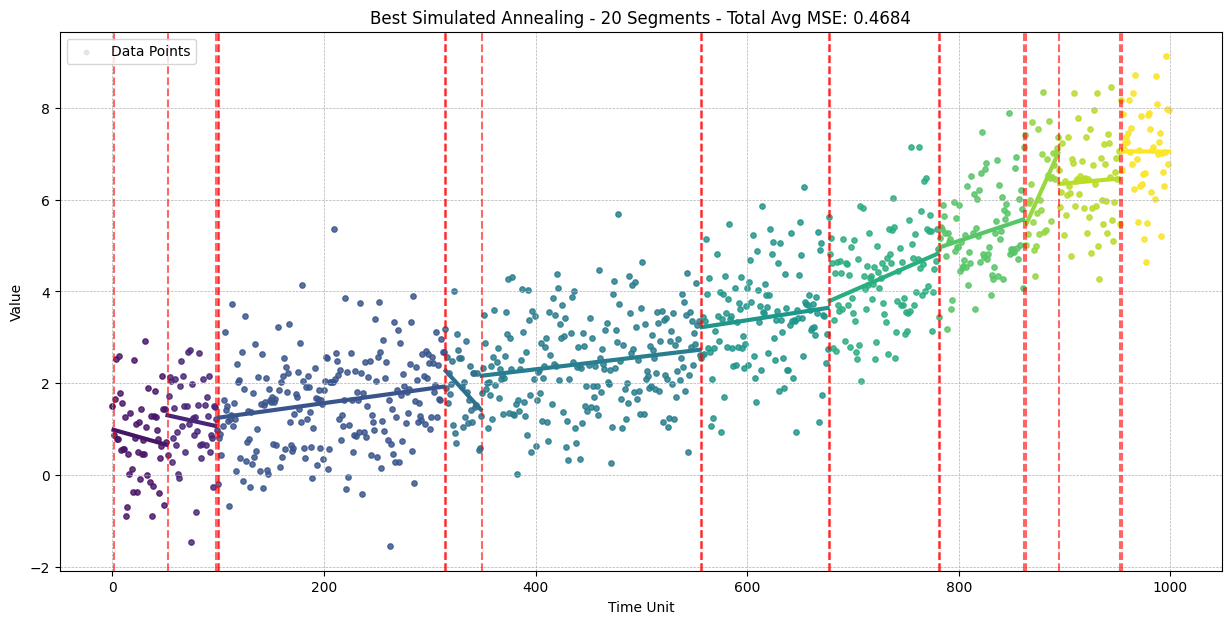
\includegraphics[width=0.85\textwidth]{img/SA-TS3.png}
  \caption{Behavioural comparison on TS3.
    Top: Random Search. Middle: Hill Climbing. Bottom: Simulated Annealing.}
  \label{fig:behav_ts3}
\end{figure}

\subsection{General Behaviour on TS4 ($k=50$)}
\begin{figure}[H]
  \centering
  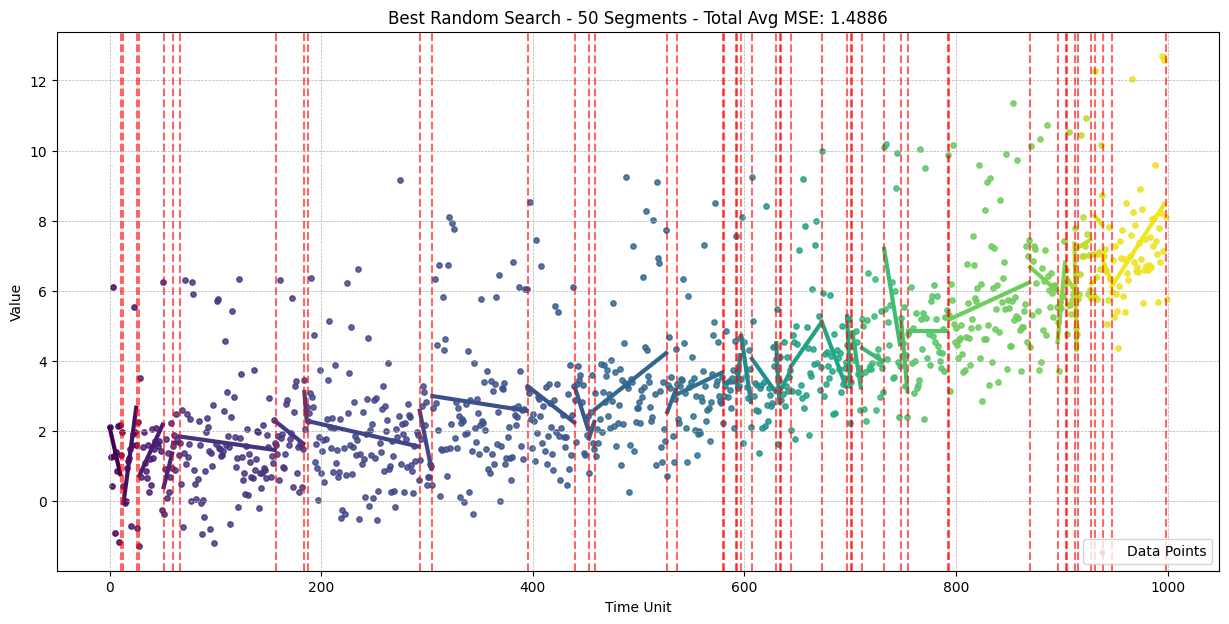
\includegraphics[width=0.85\textwidth]{img/RS-TS4.png} \\[0.3cm]
  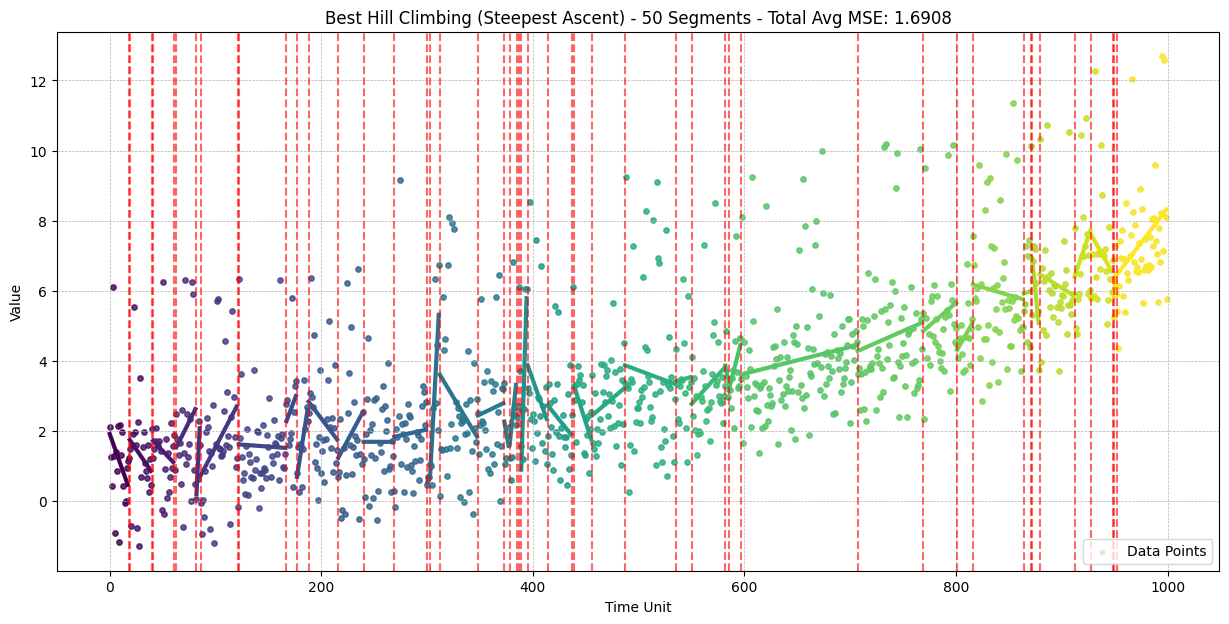
\includegraphics[width=0.85\textwidth]{img/HC-TS4.png} \\[0.3cm]
  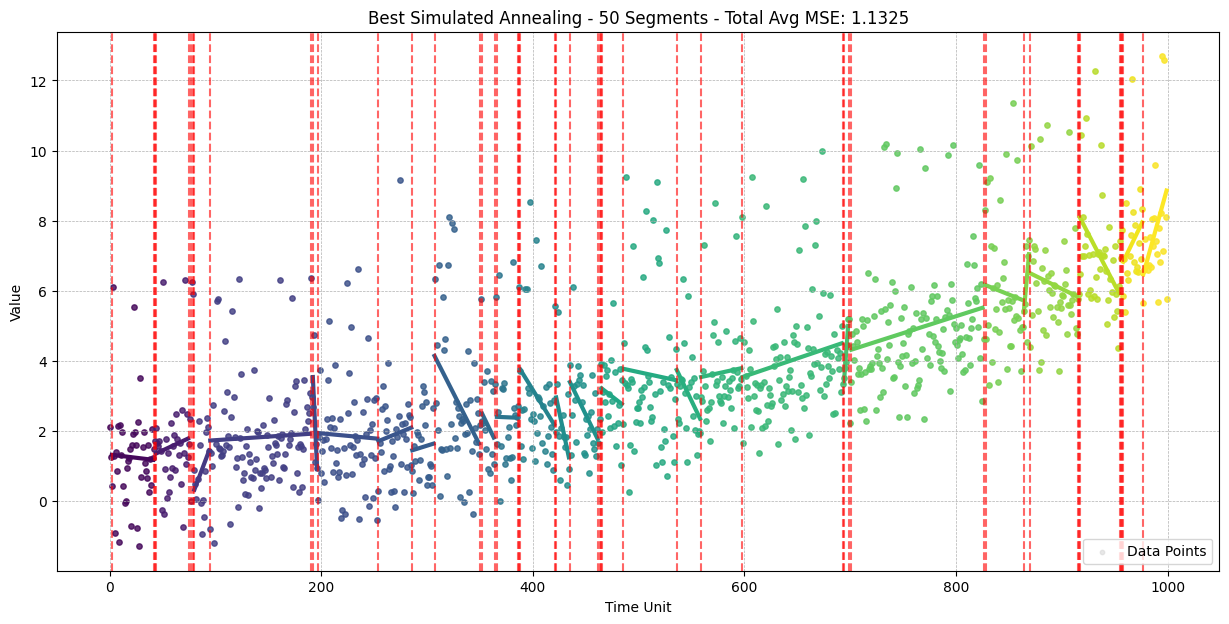
\includegraphics[width=0.85\textwidth]{img/SA-TS4.png}
  \caption{Behavioural comparison on TS4.
    Top: Random Search. Middle: Hill Climbing. Bottom: Simulated Annealing.}
  \label{fig:behav_ts4}
\end{figure}

\end{document}